\documentclass[12pt]{article}
\usepackage[utf8]{inputenc}
\usepackage[spanish]{babel}
\usepackage{graphicx}
\usepackage{amsmath}
\usepackage{amssymb}
\usepackage{array}
\usepackage{xcolor}
\usepackage{geometry}
\usepackage{fancyhdr}
\usepackage{lastpage}
\usepackage{booktabs}
\usepackage{colortbl}
\usepackage{caption}
\usepackage{multirow}
\geometry{margin=1in}

\usepackage{float}
\definecolor{lightblue}{RGB}{200,230,255}
\definecolor{lightgreen}{RGB}{220,255,220}
\definecolor{lightred}{RGB}{255,220,220}
\definecolor{lightyellow}{RGB}{255,255,200}
\pagestyle{fancy}
\fancyhf{}
\fancyhead[L]{Algoritmo de Floyd - Solución}
\fancyhead[R]{\thepage\ de \pageref{LastPage}}
\renewcommand{\headrulewidth}{0.4pt}
\renewcommand{\footrulewidth}{0.4pt}

\title{Proyecto 1: Rutas Optimas (Algoritmo de Floyd)}
\author{Emily Sanchez \\ Viviana Vargas \\[1cm] Curso: Investigación de Operaciones \\ II Semestre 2025}
\date{\today}

\begin{document}

\maketitle
\thispagestyle{empty}
\newpage
\setcounter{page}{1}

\section{Introducción}
El algoritmo de Floyd-Warshall es un algoritmo para encontrar los caminos más cortos en un grafo ponderado. Fue publicado por Robert Floyd en 1962.\\
El algoritmo de Floyd se basa en el principio de la Programación Dinámica.\\
\textbf{Complejidad espacial:} $O(n^2)$\\
\textbf{Complejidad temporal:} $O(n^3)$\\
\clearpage
\section{Descripción del Problema}
Grafo con 8 nodos:

\begin{itemize}
\item Nodo A: A
\item Nodo B: B
\item Nodo C: C
\item Nodo D: D
\item Nodo E: E
\item Nodo F: F
\item Nodo G: G
\item Nodo H: H
\end{itemize}

\begin{figure}[h!]
\centering
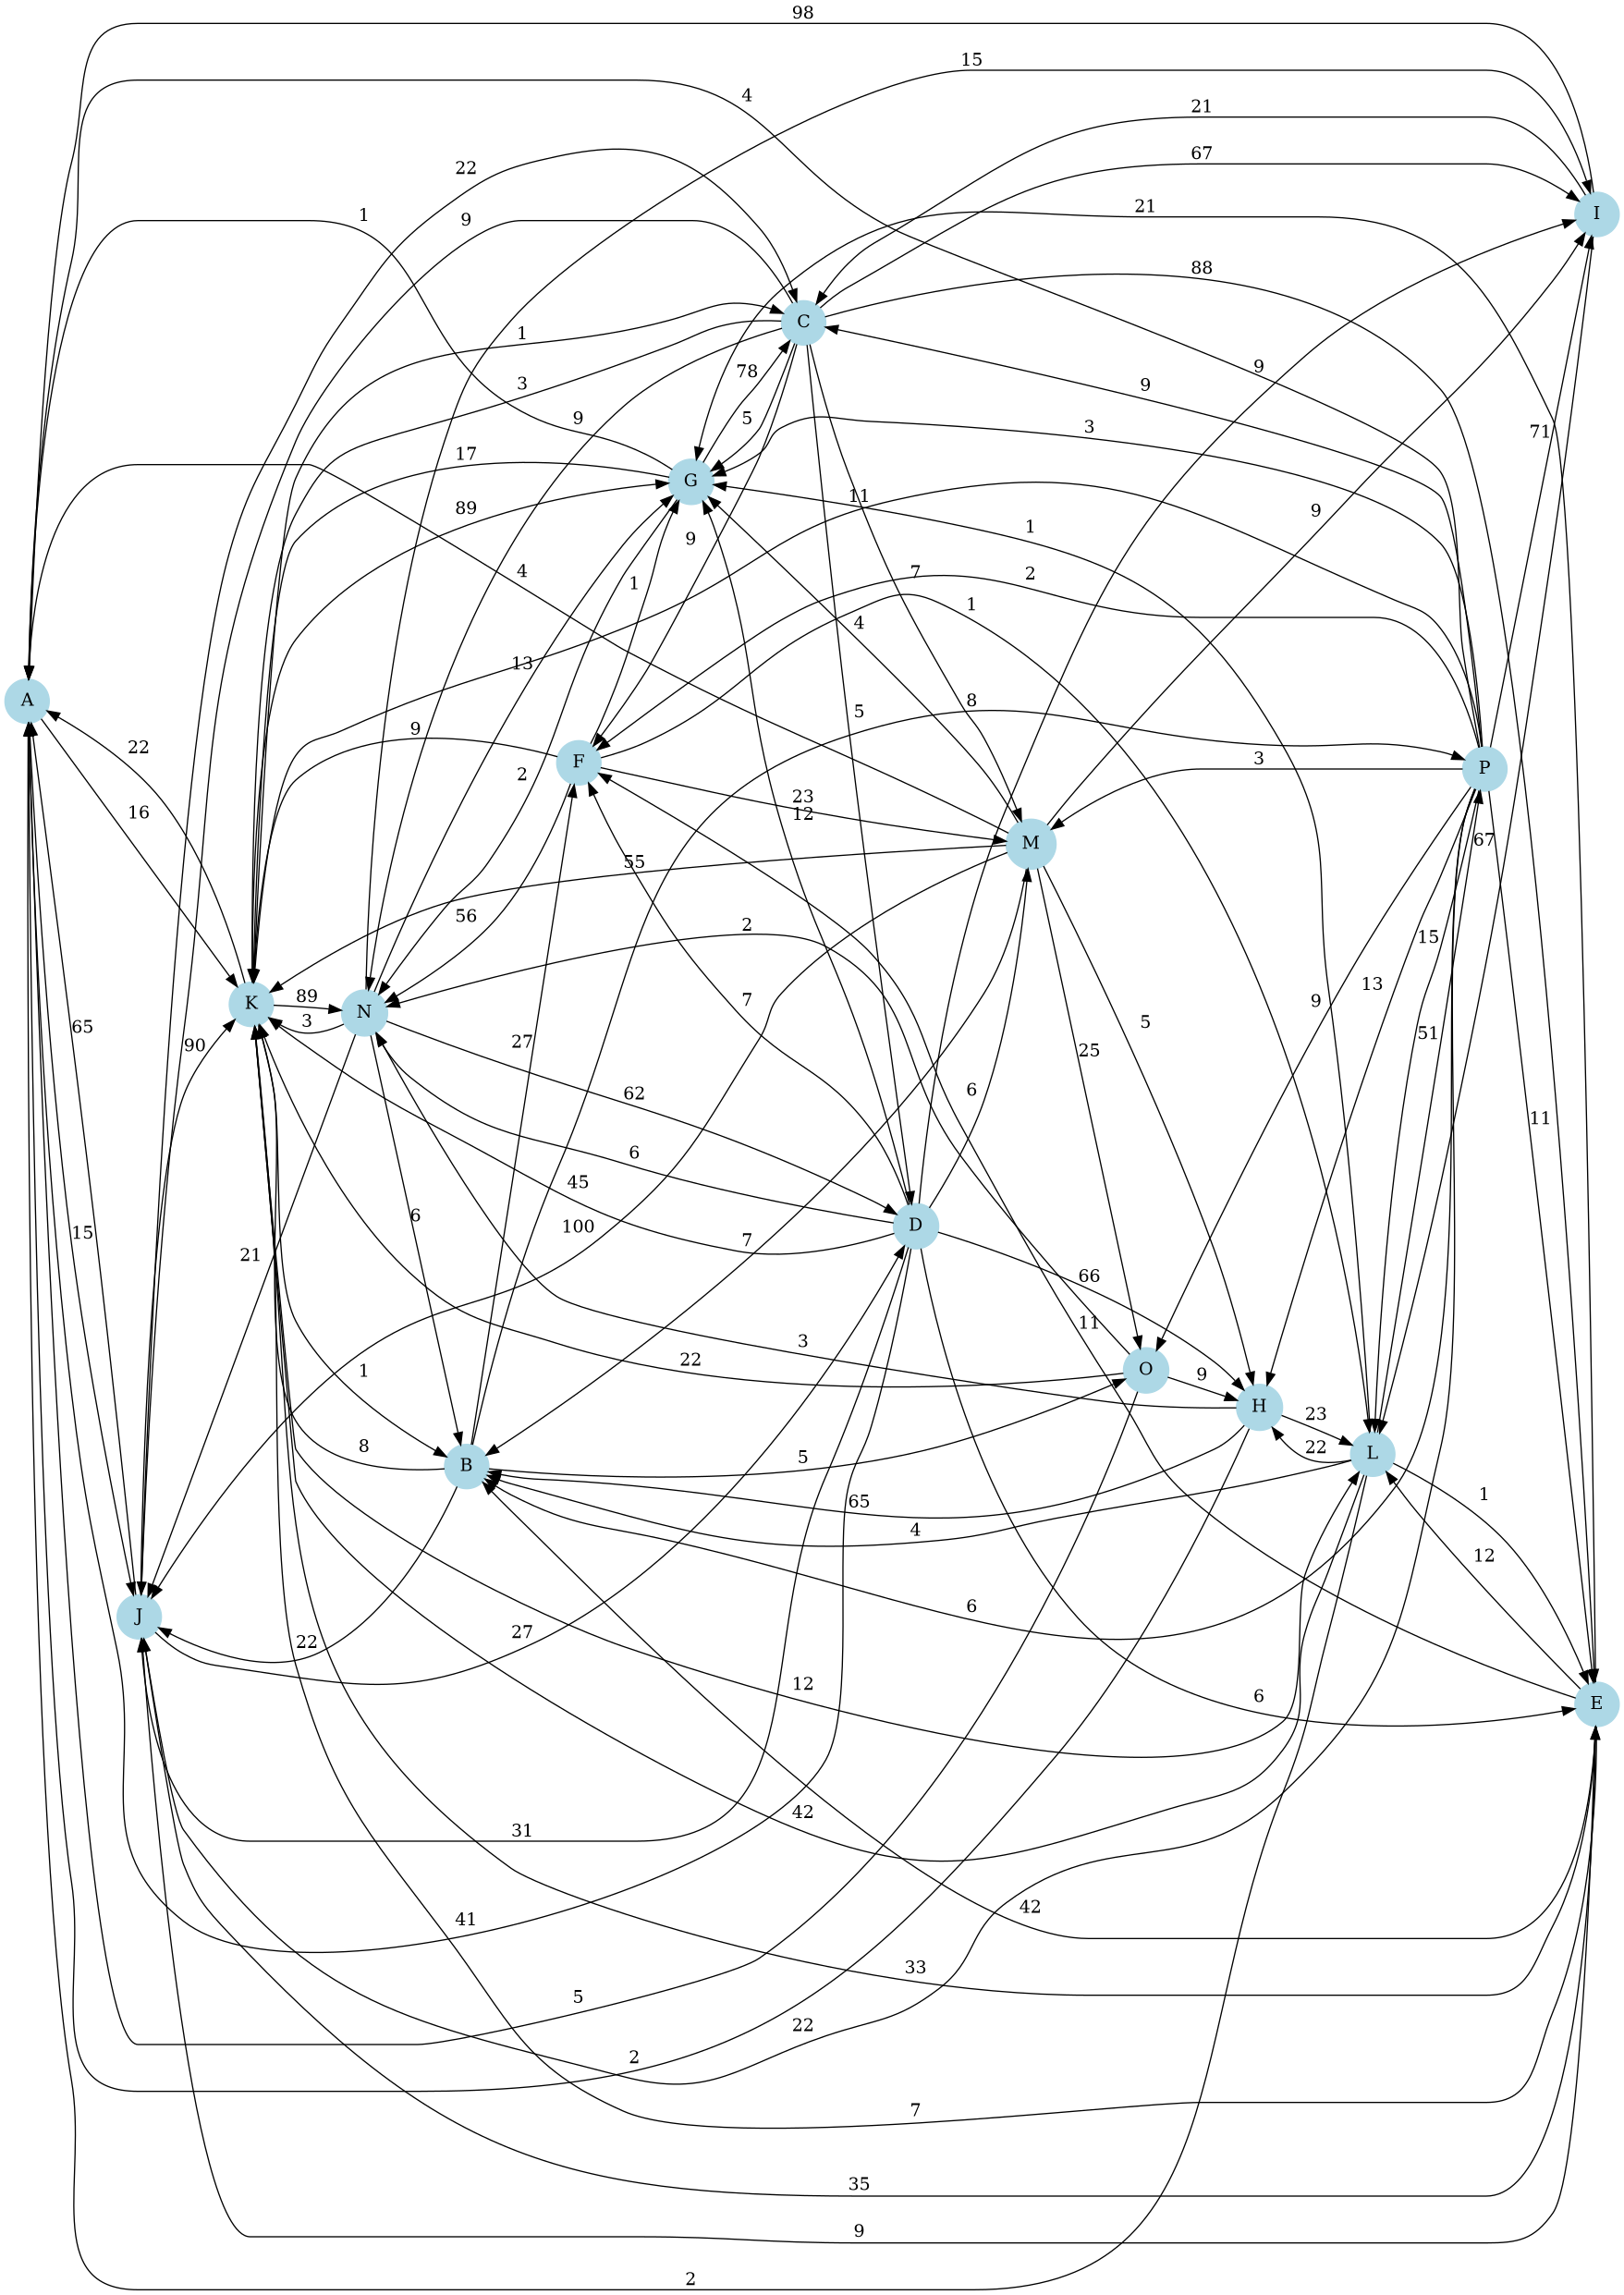
\includegraphics[width=0.5\textwidth,keepaspectratio]{grafo.png}
\caption{Representación del grafo original}
\end{figure}

\clearpage
\section{Procedimiento del Algoritmo}
\subsection{Matriz de Distancias Inicial D(0)}
\begin{table}[h!]
\centering
\begin{tabular}{|c|c|c|c|c|c|c|c|c|}
\hline
 & A & B & C & D & E & F & G & H \\\hline
A & 0 & $\infty$ & 12 & $\infty$ & $\infty$ & 65 & $\infty$ & $\infty$ \\\hline
B & 21 & 0 & 15 & 3 & $\infty$ & 1 & 6 & $\infty$ \\\hline
C & $\infty$ & 1 & 0 & $\infty$ & $\infty$ & 21 & $\infty$ & 16 \\\hline
D & 33 & 2 & 0 & 0 & $\infty$ & 12 & 7 & 8 \\\hline
E & 4 & $\infty$ & 8 & $\infty$ & 0 & 76 & 11 & $\infty$ \\\hline
F & 1 & $\infty$ & 9 & 4 & $\infty$ & 0 & $\infty$ & 10 \\\hline
G & 6 & 10 & 1 & 11 & 5 & $\infty$ & 0 & 0 \\\hline
H & 7 & $\infty$ & 26 & 21 & $\infty$ & $\infty$ & 9 & 0 \\\hline
\end{tabular}
\caption{Matriz de distancias inicial D(0)}
\end{table}

\clearpage
\subsection{Matriz de Caminos Inicial P(0)}
\begin{table}[h!]
\centering
\begin{tabular}{|c|c|c|c|c|c|c|c|c|}
\hline
 & A & B & C & D & E & F & G & H \\\hline
A & - & - & A & - & - & A & - & - \\\hline
B & B & - & B & B & - & B & B & - \\\hline
C & - & C & - & - & - & C & - & C \\\hline
D & D & D & D & - & - & D & D & D \\\hline
E & E & - & E & - & - & E & E & - \\\hline
F & F & - & F & F & - & - & - & F \\\hline
G & G & G & G & G & G & - & - & G \\\hline
H & H & - & H & H & - & - & H & - \\\hline
\end{tabular}
\caption{Matriz de caminos inicial P(0)}
\end{table}

\subsection{Iteraciones del Algoritmo}
\clearpage
\subsubsection{Iteración 1 (k = 1) - Nodo intermedio: A}
\begin{table}[h!]
\centering
\begin{tabular}{|c|c|c|c|c|c|c|c|c|}
\hline
 & A & B & C & D & E & F & G & H \\\hline
A & 0 & $\infty$ & 12 & $\infty$ & $\infty$ & 65 & $\infty$ & $\infty$ \\\hline
B & 21 & 0 & 15 & 3 & $\infty$ & 1 & 6 & $\infty$ \\\hline
C & $\infty$ & 1 & 0 & $\infty$ & $\infty$ & 21 & $\infty$ & 16 \\\hline
D & 33 & 2 & 0 & 0 & $\infty$ & 12 & 7 & 8 \\\hline
E & 4 & $\infty$ & 8 & $\infty$ & 0 & \cellcolor{lightgreen} 69 & 11 & $\infty$ \\\hline
F & 1 & $\infty$ & 9 & 4 & $\infty$ & 0 & $\infty$ & 10 \\\hline
G & 6 & 10 & 1 & 11 & 5 & \cellcolor{lightgreen} 71 & 0 & 0 \\\hline
H & 7 & $\infty$ & \cellcolor{lightgreen} 19 & 21 & $\infty$ & \cellcolor{lightgreen} 72 & 9 & 0 \\\hline
\end{tabular}
\caption{Matriz de distancias D(1) - Cambios resaltados en verde}
\end{table}

\begin{table}[h!]
\centering
\begin{tabular}{|c|c|c|c|c|c|c|c|c|}
\hline
 & A & B & C & D & E & F & G & H \\\hline
A & - & - & A & - & - & A & - & - \\\hline
B & B & - & B & B & - & B & B & - \\\hline
C & - & C & - & - & - & C & - & C \\\hline
D & D & D & D & - & - & D & D & D \\\hline
E & E & - & E & - & - & \cellcolor{lightblue} A & E & - \\\hline
F & F & - & F & F & - & - & - & F \\\hline
G & G & G & G & G & G & \cellcolor{lightblue} A & - & G \\\hline
H & H & - & \cellcolor{lightblue} A & H & - & \cellcolor{lightblue} A & H & - \\\hline
\end{tabular}
\caption{Matriz de caminos P(1) - Cambios resaltados en azul}
\end{table}

\clearpage
\subsubsection{Iteración 2 (k = 2) - Nodo intermedio: B}
\begin{table}[h!]
\centering
\begin{tabular}{|c|c|c|c|c|c|c|c|c|}
\hline
 & A & B & C & D & E & F & G & H \\\hline
A & 0 & $\infty$ & 12 & $\infty$ & $\infty$ & 65 & $\infty$ & $\infty$ \\\hline
B & 21 & 0 & 15 & 3 & $\infty$ & 1 & 6 & $\infty$ \\\hline
C & \cellcolor{lightgreen} 22 & 1 & 0 & \cellcolor{lightgreen} 4 & $\infty$ & \cellcolor{lightgreen} 2 & \cellcolor{lightgreen} 7 & 16 \\\hline
D & \cellcolor{lightgreen} 23 & 2 & 0 & 0 & $\infty$ & \cellcolor{lightgreen} 3 & 7 & 8 \\\hline
E & 4 & $\infty$ & 8 & $\infty$ & 0 & 69 & 11 & $\infty$ \\\hline
F & 1 & $\infty$ & 9 & 4 & $\infty$ & 0 & $\infty$ & 10 \\\hline
G & 6 & 10 & 1 & 11 & 5 & \cellcolor{lightgreen} 11 & 0 & 0 \\\hline
H & 7 & $\infty$ & 19 & 21 & $\infty$ & 72 & 9 & 0 \\\hline
\end{tabular}
\caption{Matriz de distancias D(2) - Cambios resaltados en verde}
\end{table}

\begin{table}[h!]
\centering
\begin{tabular}{|c|c|c|c|c|c|c|c|c|}
\hline
 & A & B & C & D & E & F & G & H \\\hline
A & - & - & A & - & - & A & - & - \\\hline
B & B & - & B & B & - & B & B & - \\\hline
C & \cellcolor{lightblue} B & C & - & \cellcolor{lightblue} B & - & \cellcolor{lightblue} B & \cellcolor{lightblue} B & C \\\hline
D & \cellcolor{lightblue} B & D & D & - & - & \cellcolor{lightblue} B & D & D \\\hline
E & E & - & E & - & - & A & E & - \\\hline
F & F & - & F & F & - & - & - & F \\\hline
G & G & G & G & G & G & \cellcolor{lightblue} B & - & G \\\hline
H & H & - & A & H & - & A & H & - \\\hline
\end{tabular}
\caption{Matriz de caminos P(2) - Cambios resaltados en azul}
\end{table}

\clearpage
\subsubsection{Iteración 3 (k = 3) - Nodo intermedio: C}
\begin{table}[h!]
\centering
\begin{tabular}{|c|c|c|c|c|c|c|c|c|}
\hline
 & A & B & C & D & E & F & G & H \\\hline
A & 0 & \cellcolor{lightgreen} 13 & 12 & \cellcolor{lightgreen} 16 & $\infty$ & \cellcolor{lightgreen} 14 & \cellcolor{lightgreen} 19 & \cellcolor{lightgreen} 28 \\\hline
B & 21 & 0 & 15 & 3 & $\infty$ & 1 & 6 & \cellcolor{lightgreen} 31 \\\hline
C & 22 & 1 & 0 & 4 & $\infty$ & 2 & 7 & 16 \\\hline
D & \cellcolor{lightgreen} 22 & \cellcolor{lightgreen} 1 & 0 & 0 & $\infty$ & \cellcolor{lightgreen} 2 & 7 & 8 \\\hline
E & 4 & \cellcolor{lightgreen} 9 & 8 & \cellcolor{lightgreen} 12 & 0 & \cellcolor{lightgreen} 10 & 11 & \cellcolor{lightgreen} 24 \\\hline
F & 1 & \cellcolor{lightgreen} 10 & 9 & 4 & $\infty$ & 0 & \cellcolor{lightgreen} 16 & 10 \\\hline
G & 6 & \cellcolor{lightgreen} 2 & 1 & \cellcolor{lightgreen} 5 & 5 & \cellcolor{lightgreen} 3 & 0 & 0 \\\hline
H & 7 & \cellcolor{lightgreen} 20 & 19 & 21 & $\infty$ & \cellcolor{lightgreen} 21 & 9 & 0 \\\hline
\end{tabular}
\caption{Matriz de distancias D(3) - Cambios resaltados en verde}
\end{table}

\begin{table}[h!]
\centering
\begin{tabular}{|c|c|c|c|c|c|c|c|c|}
\hline
 & A & B & C & D & E & F & G & H \\\hline
A & - & \cellcolor{lightblue} C & A & \cellcolor{lightblue} B & - & \cellcolor{lightblue} B & \cellcolor{lightblue} B & \cellcolor{lightblue} C \\\hline
B & B & - & B & B & - & B & B & \cellcolor{lightblue} C \\\hline
C & B & C & - & B & - & B & B & C \\\hline
D & B & \cellcolor{lightblue} C & D & - & - & B & D & D \\\hline
E & E & \cellcolor{lightblue} C & E & \cellcolor{lightblue} B & - & \cellcolor{lightblue} B & E & \cellcolor{lightblue} C \\\hline
F & F & \cellcolor{lightblue} C & F & F & - & - & \cellcolor{lightblue} B & F \\\hline
G & G & \cellcolor{lightblue} C & G & \cellcolor{lightblue} B & G & B & - & G \\\hline
H & H & \cellcolor{lightblue} C & A & H & - & \cellcolor{lightblue} B & H & - \\\hline
\end{tabular}
\caption{Matriz de caminos P(3) - Cambios resaltados en azul}
\end{table}

\clearpage
\subsubsection{Iteración 4 (k = 4) - Nodo intermedio: D}
\begin{table}[h!]
\centering
\begin{tabular}{|c|c|c|c|c|c|c|c|c|}
\hline
 & A & B & C & D & E & F & G & H \\\hline
A & 0 & 13 & 12 & 16 & $\infty$ & 14 & 19 & \cellcolor{lightgreen} 24 \\\hline
B & 21 & 0 & \cellcolor{lightgreen} 3 & 3 & $\infty$ & 1 & 6 & \cellcolor{lightgreen} 11 \\\hline
C & 22 & 1 & 0 & 4 & $\infty$ & 2 & 7 & \cellcolor{lightgreen} 12 \\\hline
D & 22 & 1 & 0 & 0 & $\infty$ & 2 & 7 & 8 \\\hline
E & 4 & 9 & 8 & 12 & 0 & 10 & 11 & \cellcolor{lightgreen} 20 \\\hline
F & 1 & \cellcolor{lightgreen} 5 & \cellcolor{lightgreen} 4 & 4 & $\infty$ & 0 & \cellcolor{lightgreen} 11 & 10 \\\hline
G & 6 & 2 & 1 & 5 & 5 & 3 & 0 & 0 \\\hline
H & 7 & 20 & 19 & 21 & $\infty$ & 21 & 9 & 0 \\\hline
\end{tabular}
\caption{Matriz de distancias D(4) - Cambios resaltados en verde}
\end{table}

\begin{table}[h!]
\centering
\begin{tabular}{|c|c|c|c|c|c|c|c|c|}
\hline
 & A & B & C & D & E & F & G & H \\\hline
A & - & C & A & B & - & B & B & \cellcolor{lightblue} D \\\hline
B & B & - & \cellcolor{lightblue} D & B & - & B & B & \cellcolor{lightblue} D \\\hline
C & B & C & - & B & - & B & B & \cellcolor{lightblue} D \\\hline
D & B & C & D & - & - & B & D & D \\\hline
E & E & C & E & B & - & B & E & \cellcolor{lightblue} D \\\hline
F & F & C & \cellcolor{lightblue} D & F & - & - & \cellcolor{lightblue} D & F \\\hline
G & G & C & G & B & G & B & - & G \\\hline
H & H & C & A & H & - & B & H & - \\\hline
\end{tabular}
\caption{Matriz de caminos P(4) - Cambios resaltados en azul}
\end{table}

\clearpage
\subsubsection{Iteración 5 (k = 5) - Nodo intermedio: E}
\begin{table}[h!]
\centering
\begin{tabular}{|c|c|c|c|c|c|c|c|c|}
\hline
 & A & B & C & D & E & F & G & H \\\hline
A & 0 & 13 & 12 & 16 & $\infty$ & 14 & 19 & 24 \\\hline
B & 21 & 0 & 3 & 3 & $\infty$ & 1 & 6 & 11 \\\hline
C & 22 & 1 & 0 & 4 & $\infty$ & 2 & 7 & 12 \\\hline
D & 22 & 1 & 0 & 0 & $\infty$ & 2 & 7 & 8 \\\hline
E & 4 & 9 & 8 & 12 & 0 & 10 & 11 & 20 \\\hline
F & 1 & 5 & 4 & 4 & $\infty$ & 0 & 11 & 10 \\\hline
G & 6 & 2 & 1 & 5 & 5 & 3 & 0 & 0 \\\hline
H & 7 & 20 & 19 & 21 & $\infty$ & 21 & 9 & 0 \\\hline
\end{tabular}
\caption{Matriz de distancias D(5) - Cambios resaltados en verde}
\end{table}

\begin{table}[h!]
\centering
\begin{tabular}{|c|c|c|c|c|c|c|c|c|}
\hline
 & A & B & C & D & E & F & G & H \\\hline
A & - & C & A & B & - & B & B & D \\\hline
B & B & - & D & B & - & B & B & D \\\hline
C & B & C & - & B & - & B & B & D \\\hline
D & B & C & D & - & - & B & D & D \\\hline
E & E & C & E & B & - & B & E & D \\\hline
F & F & C & D & F & - & - & D & F \\\hline
G & G & C & G & B & G & B & - & G \\\hline
H & H & C & A & H & - & B & H & - \\\hline
\end{tabular}
\caption{Matriz de caminos P(5) - Cambios resaltados en azul}
\end{table}

\clearpage
\subsubsection{Iteración 6 (k = 6) - Nodo intermedio: F}
\begin{table}[h!]
\centering
\begin{tabular}{|c|c|c|c|c|c|c|c|c|}
\hline
 & A & B & C & D & E & F & G & H \\\hline
A & 0 & 13 & 12 & 16 & $\infty$ & 14 & 19 & 24 \\\hline
B & \cellcolor{lightgreen} 2 & 0 & 3 & 3 & $\infty$ & 1 & 6 & 11 \\\hline
C & \cellcolor{lightgreen} 3 & 1 & 0 & 4 & $\infty$ & 2 & 7 & 12 \\\hline
D & \cellcolor{lightgreen} 3 & 1 & 0 & 0 & $\infty$ & 2 & 7 & 8 \\\hline
E & 4 & 9 & 8 & 12 & 0 & 10 & 11 & 20 \\\hline
F & 1 & 5 & 4 & 4 & $\infty$ & 0 & 11 & 10 \\\hline
G & \cellcolor{lightgreen} 4 & 2 & 1 & 5 & 5 & 3 & 0 & 0 \\\hline
H & 7 & 20 & 19 & 21 & $\infty$ & 21 & 9 & 0 \\\hline
\end{tabular}
\caption{Matriz de distancias D(6) - Cambios resaltados en verde}
\end{table}

\begin{table}[h!]
\centering
\begin{tabular}{|c|c|c|c|c|c|c|c|c|}
\hline
 & A & B & C & D & E & F & G & H \\\hline
A & - & C & A & B & - & B & B & D \\\hline
B & \cellcolor{lightblue} F & - & D & B & - & B & B & D \\\hline
C & \cellcolor{lightblue} F & C & - & B & - & B & B & D \\\hline
D & \cellcolor{lightblue} F & C & D & - & - & B & D & D \\\hline
E & E & C & E & B & - & B & E & D \\\hline
F & F & C & D & F & - & - & D & F \\\hline
G & \cellcolor{lightblue} F & C & G & B & G & B & - & G \\\hline
H & H & C & A & H & - & B & H & - \\\hline
\end{tabular}
\caption{Matriz de caminos P(6) - Cambios resaltados en azul}
\end{table}

\clearpage
\subsubsection{Iteración 7 (k = 7) - Nodo intermedio: G}
\begin{table}[h!]
\centering
\begin{tabular}{|c|c|c|c|c|c|c|c|c|}
\hline
 & A & B & C & D & E & F & G & H \\\hline
A & 0 & 13 & 12 & 16 & \cellcolor{lightgreen} 24 & 14 & 19 & \cellcolor{lightgreen} 19 \\\hline
B & 2 & 0 & 3 & 3 & \cellcolor{lightgreen} 11 & 1 & 6 & \cellcolor{lightgreen} 6 \\\hline
C & 3 & 1 & 0 & 4 & \cellcolor{lightgreen} 12 & 2 & 7 & \cellcolor{lightgreen} 7 \\\hline
D & 3 & 1 & 0 & 0 & \cellcolor{lightgreen} 12 & 2 & 7 & \cellcolor{lightgreen} 7 \\\hline
E & 4 & 9 & 8 & 12 & 0 & 10 & 11 & \cellcolor{lightgreen} 11 \\\hline
F & 1 & 5 & 4 & 4 & \cellcolor{lightgreen} 16 & 0 & 11 & 10 \\\hline
G & 4 & 2 & 1 & 5 & 5 & 3 & 0 & 0 \\\hline
H & 7 & \cellcolor{lightgreen} 11 & \cellcolor{lightgreen} 10 & \cellcolor{lightgreen} 14 & \cellcolor{lightgreen} 14 & \cellcolor{lightgreen} 12 & 9 & 0 \\\hline
\end{tabular}
\caption{Matriz de distancias D(7) - Cambios resaltados en verde}
\end{table}

\begin{table}[h!]
\centering
\begin{tabular}{|c|c|c|c|c|c|c|c|c|}
\hline
 & A & B & C & D & E & F & G & H \\\hline
A & - & C & A & B & \cellcolor{lightblue} G & B & B & \cellcolor{lightblue} G \\\hline
B & F & - & D & B & \cellcolor{lightblue} G & B & B & \cellcolor{lightblue} G \\\hline
C & F & C & - & B & \cellcolor{lightblue} G & B & B & \cellcolor{lightblue} G \\\hline
D & F & C & D & - & \cellcolor{lightblue} G & B & D & \cellcolor{lightblue} G \\\hline
E & E & C & E & B & - & B & E & \cellcolor{lightblue} G \\\hline
F & F & C & D & F & \cellcolor{lightblue} G & - & D & F \\\hline
G & F & C & G & B & G & B & - & G \\\hline
H & H & C & \cellcolor{lightblue} G & \cellcolor{lightblue} B & \cellcolor{lightblue} G & B & H & - \\\hline
\end{tabular}
\caption{Matriz de caminos P(7) - Cambios resaltados en azul}
\end{table}

\clearpage
\subsubsection{Iteración 8 (k = 8) - Nodo intermedio: H}
\begin{table}[h!]
\centering
\begin{tabular}{|c|c|c|c|c|c|c|c|c|}
\hline
 & A & B & C & D & E & F & G & H \\\hline
A & 0 & 13 & 12 & 16 & 24 & 14 & 19 & 19 \\\hline
B & 2 & 0 & 3 & 3 & 11 & 1 & 6 & 6 \\\hline
C & 3 & 1 & 0 & 4 & 12 & 2 & 7 & 7 \\\hline
D & 3 & 1 & 0 & 0 & 12 & 2 & 7 & 7 \\\hline
E & 4 & 9 & 8 & 12 & 0 & 10 & 11 & 11 \\\hline
F & 1 & 5 & 4 & 4 & 16 & 0 & 11 & 10 \\\hline
G & 4 & 2 & 1 & 5 & 5 & 3 & 0 & 0 \\\hline
H & 7 & 11 & 10 & 14 & 14 & 12 & 9 & 0 \\\hline
\end{tabular}
\caption{Matriz de distancias D(8) - Cambios resaltados en verde}
\end{table}

\begin{table}[h!]
\centering
\begin{tabular}{|c|c|c|c|c|c|c|c|c|}
\hline
 & A & B & C & D & E & F & G & H \\\hline
A & - & C & A & B & G & B & B & G \\\hline
B & F & - & D & B & G & B & B & G \\\hline
C & F & C & - & B & G & B & B & G \\\hline
D & F & C & D & - & G & B & D & G \\\hline
E & E & C & E & B & - & B & E & G \\\hline
F & F & C & D & F & G & - & D & F \\\hline
G & F & C & G & B & G & B & - & G \\\hline
H & H & C & G & B & G & B & H & - \\\hline
\end{tabular}
\caption{Matriz de caminos P(8) - Cambios resaltados en azul}
\end{table}

\clearpage
\section{Resultados Finales}
\subsection{Matriz de Distancias Final D(8)}
\begin{table}[h!]
\centering
\begin{tabular}{|c|c|c|c|c|c|c|c|c|}
\hline
 & A & B & C & D & E & F & G & H \\\hline
A & 0 & 13 & 12 & 16 & 24 & 14 & 19 & 19 \\\hline
B & 2 & 0 & 3 & 3 & 11 & 1 & 6 & 6 \\\hline
C & 3 & 1 & 0 & 4 & 12 & 2 & 7 & 7 \\\hline
D & 3 & 1 & 0 & 0 & 12 & 2 & 7 & 7 \\\hline
E & 4 & 9 & 8 & 12 & 0 & 10 & 11 & 11 \\\hline
F & 1 & 5 & 4 & 4 & 16 & 0 & 11 & 10 \\\hline
G & 4 & 2 & 1 & 5 & 5 & 3 & 0 & 0 \\\hline
H & 7 & 11 & 10 & 14 & 14 & 12 & 9 & 0 \\\hline
\end{tabular}
\caption{Matriz de distancias final D(8)}
\end{table}

\clearpage
\subsection{Matriz de Caminos Final P(8)}
\begin{table}[h!]
\centering
\begin{tabular}{|c|c|c|c|c|c|c|c|c|}
\hline
 & A & B & C & D & E & F & G & H \\\hline
A & - & C & A & B & G & B & B & G \\\hline
B & F & - & D & B & G & B & B & G \\\hline
C & F & C & - & B & G & B & B & G \\\hline
D & F & C & D & - & G & B & D & G \\\hline
E & E & C & E & B & - & B & E & G \\\hline
F & F & C & D & F & G & - & D & F \\\hline
G & F & C & G & B & G & B & - & G \\\hline
H & H & C & G & B & G & B & H & - \\\hline
\end{tabular}
\caption{Matriz de caminos final P(8)}
\end{table}

\clearpage
\subsection{Rutas Óptimas}
\begin{itemize}
\item \textbf{A → B:} Distancia: 13, Ruta: A → C → B
\item \textbf{A → C:} Distancia: 12, Ruta: A → C
\item \textbf{A → D:} Distancia: 16, Ruta: A → C → B → D
\item \textbf{A → E:} Distancia: 24, Ruta: A → C → B → G → E
\item \textbf{A → F:} Distancia: 14, Ruta: A → C → B → F
\item \textbf{A → G:} Distancia: 19, Ruta: A → C → B → G
\item \textbf{A → H:} Distancia: 19, Ruta: A → C → B → G → H
\item \textbf{B → A:} Distancia: 2, Ruta: B → F → A
\item \textbf{B → C:} Distancia: 3, Ruta: B → D → C
\item \textbf{B → D:} Distancia: 3, Ruta: B → D
\item \textbf{B → E:} Distancia: 11, Ruta: B → G → E
\item \textbf{B → F:} Distancia: 1, Ruta: B → F
\item \textbf{B → G:} Distancia: 6, Ruta: B → G
\item \textbf{B → H:} Distancia: 6, Ruta: B → G → H
\item \textbf{C → A:} Distancia: 3, Ruta: C → B → F → A
\item \textbf{C → B:} Distancia: 1, Ruta: C → B
\item \textbf{C → D:} Distancia: 4, Ruta: C → B → D
\item \textbf{C → E:} Distancia: 12, Ruta: C → B → G → E
\item \textbf{C → F:} Distancia: 2, Ruta: C → B → F
\item \textbf{C → G:} Distancia: 7, Ruta: C → B → G
\item \textbf{C → H:} Distancia: 7, Ruta: C → B → G → H
\item \textbf{D → A:} Distancia: 3, Ruta: D → C → B → F → A
\item \textbf{D → B:} Distancia: 1, Ruta: D → C → B
\item \textbf{D → C:} Distancia: 0, Ruta: D → C
\item \textbf{D → E:} Distancia: 12, Ruta: D → G → E
\item \textbf{D → F:} Distancia: 2, Ruta: D → C → B → F
\item \textbf{D → G:} Distancia: 7, Ruta: D → G
\item \textbf{D → H:} Distancia: 7, Ruta: D → G → H
\item \textbf{E → A:} Distancia: 4, Ruta: E → A
\item \textbf{E → B:} Distancia: 9, Ruta: E → C → B
\item \textbf{E → C:} Distancia: 8, Ruta: E → C
\item \textbf{E → D:} Distancia: 12, Ruta: E → C → B → D
\item \textbf{E → F:} Distancia: 10, Ruta: E → C → B → F
\item \textbf{E → G:} Distancia: 11, Ruta: E → G
\item \textbf{E → H:} Distancia: 11, Ruta: E → G → H
\item \textbf{F → A:} Distancia: 1, Ruta: F → A
\item \textbf{F → B:} Distancia: 5, Ruta: F → D → C → B
\item \textbf{F → C:} Distancia: 4, Ruta: F → D → C
\item \textbf{F → D:} Distancia: 4, Ruta: F → D
\item \textbf{F → E:} Distancia: 16, Ruta: F → D → G → E
\item \textbf{F → G:} Distancia: 11, Ruta: F → D → G
\item \textbf{F → H:} Distancia: 10, Ruta: F → H
\item \textbf{G → A:} Distancia: 4, Ruta: G → C → B → F → A
\item \textbf{G → B:} Distancia: 2, Ruta: G → C → B
\item \textbf{G → C:} Distancia: 1, Ruta: G → C
\item \textbf{G → D:} Distancia: 5, Ruta: G → C → B → D
\item \textbf{G → E:} Distancia: 5, Ruta: G → E
\item \textbf{G → F:} Distancia: 3, Ruta: G → C → B → F
\item \textbf{G → H:} Distancia: 0, Ruta: G → H
\item \textbf{H → A:} Distancia: 7, Ruta: H → A
\item \textbf{H → B:} Distancia: 11, Ruta: H → G → C → B
\item \textbf{H → C:} Distancia: 10, Ruta: H → G → C
\item \textbf{H → D:} Distancia: 14, Ruta: H → G → C → B → D
\item \textbf{H → E:} Distancia: 14, Ruta: H → G → E
\item \textbf{H → F:} Distancia: 12, Ruta: H → G → C → B → F
\item \textbf{H → G:} Distancia: 9, Ruta: H → G
\end{itemize}
\end{document}
